\documentclass[UTF8]{ctexart}
\author{李昂}
\title{基于统计回归的地震破坏性分析模型及东日本大地震仙台市灾情分析中的应用}
\usepackage{amsmath}
\usepackage{amssymb}
\usepackage{url}
\usepackage{geometry}
\usepackage{appendix}
\usepackage{booktabs}
\usepackage{cases}
\usepackage{graphicx}
\usepackage{subfigure}
\usepackage{listings}
\usepackage{xcolor}
\usepackage{fancyhdr}

\pagestyle{fancy}
\lhead{}
\chead{}
\rhead{}
\lfoot{}
\cfoot{\thepage}
\rfoot{}
\renewcommand{\headrulewidth}{0pt}
\renewcommand{\footrulewidth}{0pt}

\linespread{1.5}
\geometry{left=2.5cm,right=2.5cm,top=2.5cm,bottom=2.5cm}
\bibliographystyle{gbt7714-2005}

\begin{document}
\maketitle
\begin{abstract}
东京时间 2011 年 3 月 11 日 14 时 46 分,日本东北地方太平洋海域发生里氏 9.0 级地震,并伴随有 7.0 到 7.4 级的多次强余震。9.0 级地震也造成了历史记录以来罕见的高达 39 米的巨大海啸。截止到 2011 年 5 月,超过 2.4 万人被官方报告为死亡或失踪;另外,福岛第一核电站因此发生的严重核事故也导致了千余人的非直接死亡,这些一并发生的重大事故也给日本及周边国家带来了严重的损失。本文通过评估磐城、仙台、宫古与横须贺的地震破坏及损失情况,利用多元线性回归的方式,建立了灾害有关因素(地震强度、海啸等)与灾害造成的后果(人员伤亡、经济损失)的模型。

本文根据互联网中能够查得的数据进行提取,并获得了沿岸海浪最大高度、与震中距离、地震里氏烈度、经济水平(GDP)等数据,以及人员伤亡、财产损失的数据。根据绘制的散点图确定多元拟合中每个分量对应的多项式次数,之后将高次单项式换元转化为一次单项式,使用多元线性拟合来得出多项式系数。利用所得出的模型,本文又简要分析了仙台市的灾情情况,并且指出数据点较少带来的模型的不足之处。
\begin{flushleft}
\textbf{关键词:} 多项式拟合; 地震破坏性评估; 东日本大地震
\end{flushleft}
\end{abstract}

\clearpage

\section{问题背景与分析}
\subsection{背景}
2011 年 3 月 11 日日本福岛发生里氏 9.0 级大地震,强震引发海啸,导致当时全球最大的在役核电站——福岛核电站放射性物质外泄。该事故根据国际核事件分级被评为最高级 7 级,与切尔诺贝利核电站泄漏事故等级相同。截至 2014 年 2 月,“3.11”东日本大地震和大海啸死亡的人数达到 15884 人。截至 2014 年 5 月,受东日本大地震和福岛第一核电站事故影响,非直接死亡的人数已经达到 1699 人,超过了在事故中直接死亡的 1603 人。

建立数学模型,在以下日本沿海城市:磐城、仙台、宫古和横须贺中。比较各种规模大小的地震破坏以及所造成的后果,并为当地报纸准备一篇文章,解释根据你的模型关于其中一个城市的发现。

\subsection{问题分析}
该问题本质为求解一个地震因子向量$x = (x_1, x_2, ..., x_m)$到影响程度向量$y = (y_1, y_2, ..., y_n)$的函数$F$(可能包含多个线性变换),表示为
$$y = F(x)$$
,怎样得出$F(x)$也是本文讨论的核心内容。

由于灾害产生的影响与人类生产力水平的发展情况和人自身的主观能动性有很大的关联,所以单纯凭借历史以来的地震伤亡人数、财产损失情况不能作为衡量当今灾害情况与财产损失的直接依据,但是人类自身因素又是衡量地震带来的破坏性的必要考虑因素,且关系极其复杂。为了简化模型、提高模型准确性与说服力,我们将磐城、仙台、宫古和横须贺四个地区在同一时间横向对比,不需控制时间的变量,而是通过与震中的距离来衡量地震的影响规模。

题目所给出的四个地区的建设、经济发展水平不尽相同。图 1 是 Google Maps 的数据,给出了四城的地理位置与震中坐标,最右侧海域中的是本次地震的震中,其余点从上到下依次为宫古、仙台、磐城、横须贺;

\begin{figure}[htbp]
  \centering
  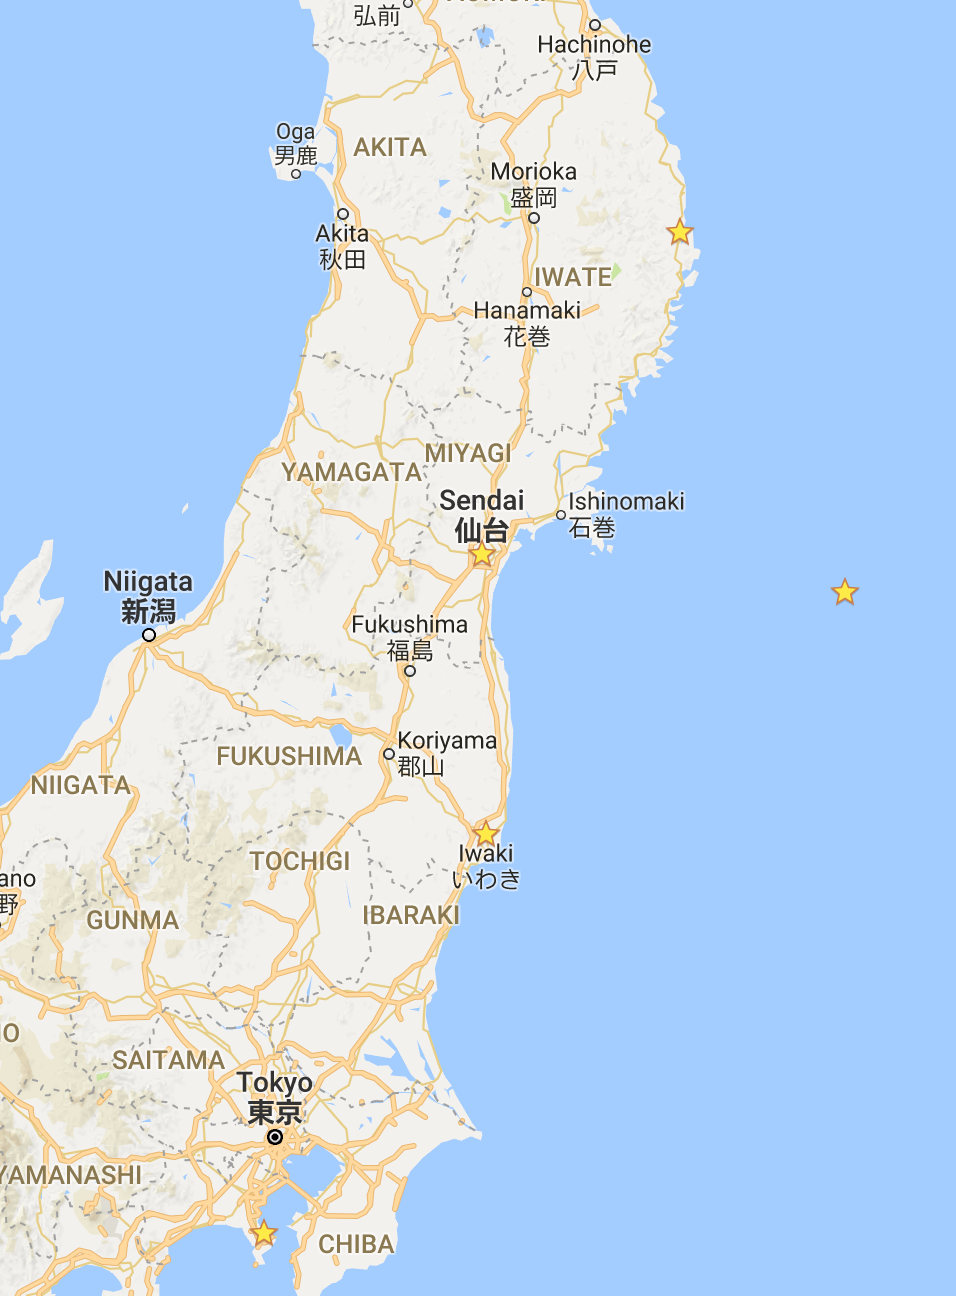
\includegraphics[width=0.95\textwidth]{../images/gmaps.png}
  \caption{Google Maps 数据}
  \label{fig:shapes}
\end{figure}

以及四城 2010 年当时的国民生产总值(GDP)\cite{宮古市役所2011財政状況資料集}\cite{横須賀市財政白書(平成23年度決算)}\cite{Kanemoto2010SendaiGDP}\cite{いわき市役所平成23年度決算}:

\begin{table}[htbp]
  \caption{2010 年四城国民生产总值(单位:亿美元)}
  \label{tab:sample}
  \centering
  \begin{tabular}{lr}
    城市 & 国民生产总值 \\
    仙台 & 61.7 \\
    横须贺 & 12.2882 \\
    磐城 & 16.5905 \\
    宫古 & 5.19
  \end{tabular}
\end{table}

由此我们将经济因素(代表抗灾、救灾水平)纳入到考虑因素中。除此之外,根据常识,地震破坏性本身又与震中位置、震源深度以及城市与震中的距离相关,也是模型中必要的考虑因素。Google Maps 分别提供了四城市中心到震中的直线距离(表 \ref{tab:distanceToCenter});

\begin{table}[htbp]
  \centering
  \caption{震中直线距离}
  \label{tab:distanceToCenter}
  \begin{tabular}{ll}
    \hline
    城市  & 与震中距离 / km \\ \hline
    宫古  & 186.45     \\
    仙台  & 176.75     \\
    磐城  & 207.31     \\
    横须贺 & 423.28     \\ \hline
  \end{tabular}
\end{table}

此外,连带因素还包括由于日本部分区域近海而产生的由地震引发的海啸影响、以及福岛核电站放射性物质外泄造成的事故。四个城市的海啸浪高度最大值可以在气象数据中查得\cite{JMA2011TsunamiHeight}\cite{JMATsunamiSites}(表 \ref{tab:tsunamiHeight});\footnote{部分观测点不以城市命名,选取对应最近的观测点。}以及从各城市与所属县政府查得的人员伤亡与财产损失情况(表 \ref{tab:earthquakeResults})\cite{Miyako2015EarthquakeTsunamiRecord}\cite{仙台市役所2017Report}\cite{いわき市役所2015災害対策本部週報}\cite{横須賀市2011東日本大震災関連情報}。

\begin{table}[htbp]{}
  \centering
  \caption{观测到的海啸高度}
  \label{tab:tsunamiHeight}
  \begin{tabular}{ll}
    \hline
    城市  & 海啸沿岸最大高度 / 米 \\ \hline
    宫古  & 8.5          \\
    仙台  & 8.6          \\
    磐城  & 6.51         \\
    横须贺 & 2.06         \\ \hline
  \end{tabular}
\end{table}

\begin{table}[htbp]
  \centering
  \caption{四城伤亡人数与经济损失}
  \label{tab:earthquakeResults}
  \begin{tabular}{lll}
    \hline
    城市  & 伤亡人数 & 经济损失(亿美元) \\ \hline
    宫古  & 611  & 22.4775   \\
    仙台  & 904  & 119.0022  \\
    横须贺 & 0    & 0.92      \\
    磐城  & 466  & 0.1478    \\ \hline
  \end{tabular}
\end{table}

\section{模型假设与说明}
\subsection{符号说明}
详见表 \ref{tab:symbolDescription}。
\begin{table}[htbp]
  \caption{本文所使用的符号说明}
  \label{tab:symbolDescription}
  \centering
  \begin{tabular}{@{}ll@{}}
    \toprule
    符号 & 代表意义与说明 \\ \midrule
    $A_1$ & 仙台市 \\
    $A_2$ & 横须贺市 \\
    $A_3$ & 宫古市 \\
    $A_4$ & 磐城市 \\
    $X$ & 表示地震整体因素的向量 \\
    $x_1, ..., x_m$ & 影响地震破坏性的各个因素 \\
    $Y$ & 表示地震破坏性结果的向量 \\
    $y_1, ..., y_n$ & 地震破坏程度的不同衡量特征(财产损失等)\\
    $F$ & 最终求解的地震破坏性衡量函数 \\
    $d_1, ..., d_4$ & 对应 $A_1, ..., A_4$ 到震中的直线距离,单位为千米 \\ \bottomrule
  \end{tabular}
\end{table}

\subsection{模型假设}
假设 1:日本本土海岸线在地震中没有大规模(超过 10 米的显著)偏移;\cite{NASA2011JapanMoving}

假设 2:人类的能动性(主观性与生产力)与发展时间相关且满足映射关系;

假设 3:人类在地震中的抗灾防灾水平与经济发展程度正相关;

假设 4:一个城市区域内的建筑物强度可以用一个平均值来表示,且可以用建筑物的强度、破坏程度作为衡量城市破坏程度的主要因素。

\section{模型建立}
\subsection{知识背景}
\subsubsection{地震影响场}
采用的地震烈度影响场衰减公式:

沿长轴方向,$I_a = 3.6345 + 1.6124M - 1.7106\ln(d + 20), \delta_{Ia} = 0.474$;

沿短轴方向,$I_b = 2.7030 + 1.5779M - 1.5407\ln(d + 20), \delta_{Ib} = 0.493$,

其中 $d$ 表示城市与震中的直线距离。\cite{傅再扬2007福建地震灾害损失计算分析与思考}

\subsubsection{海啸等级}
采用太平洋地区普遍适用的今村-饭田强度分级来评定海啸的强度等级,其中 $H_{av}$ 表示沿最近海岸的平均海啸高度,$I$ 为输出强度值。\cite{papadopoulos2001proposal}

$$I = \frac{1}{2} + \log_{2}H_{av}$$

\subsection{具体问题参数引入}
由问题分析所述,已经基本可以确定 $X$、$Y$ 各分量的表示含义。将$x_1, x_2, y_1, ...$等分量指派为表 \ref{tab:xDescription}、\ref{tab:yDescription} 中所示的含义;四城中每个城市都与且仅与一组向量对应。
\begin{table}[htbp]
  \caption{地震影响因子向量 $x$ 各分量表示含义}
  \label{tab:xDescription}
  \centering
  \begin{tabular}{lr}
    维度 & 表示含义与单位说明 \\
    $x_1$ & 地震震级(里氏) \\
    $x_2$ & 国民生产总值(亿美元)\\
    $x_3$ & 输入值在 $d_1, ..., d_4$ 范围内,与震中直线距离(千米)\\
    $x_4$ & 海啸沿岸最大高度(米)
  \end{tabular}
\end{table}

\begin{table}[htbp]
  \centering
  \caption{影响结果 $y$ 各分量表示含义}
  \label{tab:yDescription}
  \begin{tabular}{lr}
    维度    & 表示含义与单位说明 \\
    $y_1$ & 伤亡人数      \\
    $y_2$ & 经济损失(亿美元)
  \end{tabular}
\end{table}

并通过 Python 语言与 Matplotlib 库绘制 $y$ 各分量与 $x$ 各分量散点图:

\begin{figure}[htbp]
  \begin{minipage}[t]{0.5\linewidth}
    \centering
    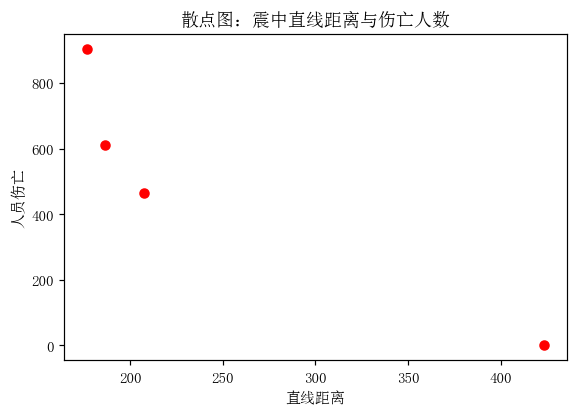
\includegraphics[width=3in]{../images/scatter-distance-person.png}
    \label{fig:scatter:distance-person}
    \caption{震中距离与伤亡人数}
  \end{minipage}
  \begin{minipage}[t]{0.5\linewidth}
    \centering
    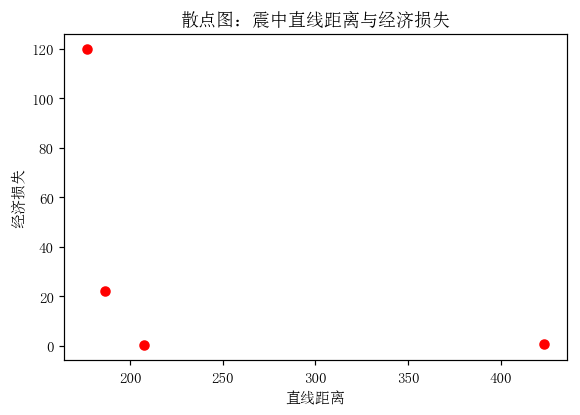
\includegraphics[width=3in]{../images/scatter-distance-economy.png}
    \label{fig:scatter:distance-economy}
    \caption{震中距离与经济损失}
\end{minipage}
\end{figure}

\begin{figure}[htbp]
  \begin{minipage}[t]{0.5\linewidth}
    \centering
    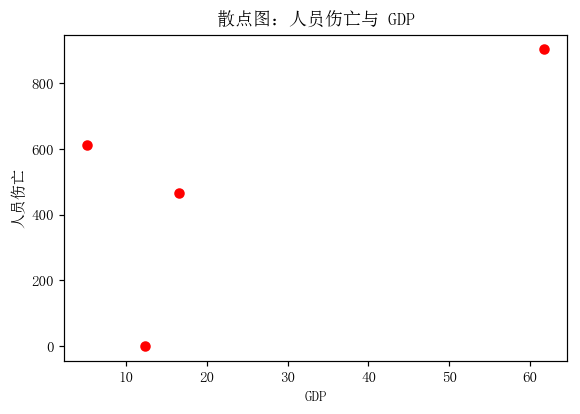
\includegraphics[width=3in]{../images/scatter-gdp-person.png}
    \label{fig:scatter:gdp-person}
    \caption{GDP 与伤亡人数}
  \end{minipage}
  \begin{minipage}[t]{0.5\linewidth}
    \centering
    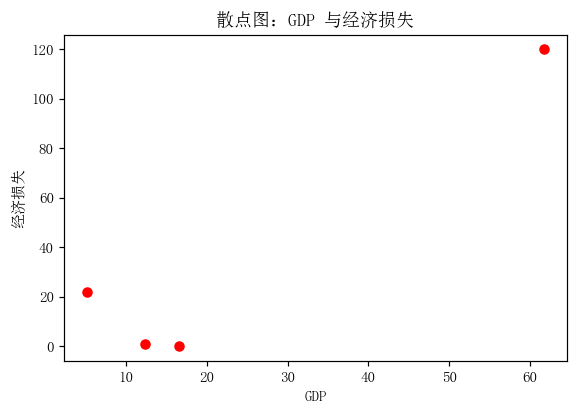
\includegraphics[width=3in]{../images/scatter-gdp-economy.png}
    \label{fig:scatter:gdp-economy}
    \caption{GDP 与经济损失}
\end{minipage}
\end{figure}

\begin{figure}[htbp]
  \begin{minipage}[t]{0.5\linewidth}
    \centering
    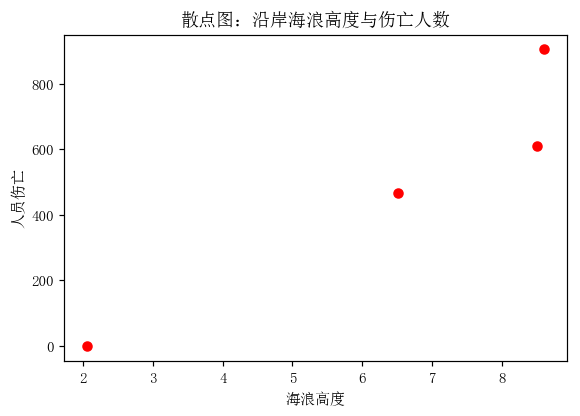
\includegraphics[width=3in]{../images/scatter-tsunami-person.png}
    \label{fig:scatter:tsunami-person}
    \caption{海浪高度与伤亡人数}
  \end{minipage}
  \begin{minipage}[t]{0.5\linewidth}
    \centering
    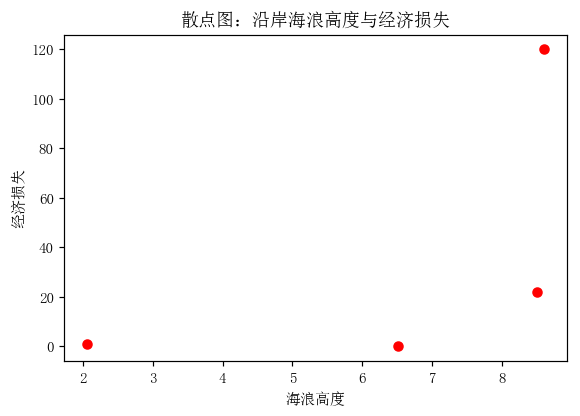
\includegraphics[width=3in]{../images/scatter-tsunami-economy.png}
    \label{fig:scatter:tsunami-economy}
    \caption{海浪高度与经济损失}
\end{minipage}
\end{figure}

\subsection{基本模型}
根据现有散点图及统计回归模型,认为 $y_1, y_2$ 为被解释变量,$x_1, ..., x_4$ 为解释变量。观察散点图,认为 $y_1$ 与 $x_3$,$y_2$ 与 $x_3$ 满足二次多项式拟合的图像特征,且函数对应单调递减:
$$y_1 = a_{30} + a_{31}x_3 + a_{32}x_3^2$$
$$y_2 = b_{30} + b_{31}x_3 + b_{32}x_3^2$$
其中 $a_{ij}, b_{ij}$ 为需要求出的多项式系数,$i = 1, 2, 3, 4$,$j = 0, 1, 2$,而且拟合曲线应当单调递减。类似方法可得 $y_1$ 与 $x_2$、$y_2$ 与 $x_2$ 线性关系,
$$y_1 = a_{20} + a_{21}x_2$$
$$y_2 = b_{20} + b_{21}x_2$$
以及 $y_1$ 与 $x_4$, $y_2$ 与 $x_4$ 的图像特征也可用二次多项式来拟合:
$$y_1 = a_{40} + a_{41}x_4 + a_{42}x_4^2$$
$$y_2 = b_{40} + b_{41}x_4 + b_{42}x_4^2$$
$y_1$ 与 $y_2$ 的取值受到以上因素的影响。所以可以得出关于 $x_2, x_3, x_4$ 的两个三元多项式拟合函数
$$
\left\{
\begin{array}{rcl}
y_1 & = & c_1 + a_{31}x_3 + a_{32}x_3^2 + a_{21}x_2 + a_{41}x_4 + a_{42}x_4^2\quad(1) \\
y_2 & = & c_2 + b_{31}x_3 + b_{32}x_3^2 + b_{21}x_2 + b_{41}x_4 + b_{42}x_4^2\quad(2)
\end{array}
\right.
$$
,其中 $c_1$,$c_2$ 为该多项式拟合模型中的常数,也就是
$$c_1 = a_{30} + a_{20} + a_{40}$$
$$c_2 = b_{30} + b_{20} + b_{40}$$

\section{模型求解}

引入拟合方法中的最小二乘法,使用多元线性回归的方法求解该模型。

令 $x_5 = x_3^2$,$x_6 = x_4^2$,此时原函数变为五元线性拟合。
$$
\left\{
\begin{array}{rcl}
y_1 & = & c_1 + a_{31}x_3 + a_{32}x_5 + a_{21}x_2 + a_{41}x_4 + a_{42}x_6\quad(1) \\
y_2 & = & c_2 + b_{31}x_3 + b_{32}x_5 + b_{21}x_2 + b_{41}x_4 + b_{42}x_6\quad(2)
\end{array}
\right.
$$
对于任意一个取值点 $(x_{ij}, y_{kj})$,其中 $j = 0, ..., 3$,$i = 1, ..., 6$,$k = 1, 2$(已知四个城市对应的数据点),有
$$y_{kj} = c_{kj} + a_{31}x_{3j} + a_{32}x_{5j} + a_{21}x_{2j} + a_{41}x_{4j} + a_{42}x_{6j}$$
,对于 $y_1$,也就是
$$
\left\{
\begin{array}{rcl}
y_{10} & = & c_1 + a_{31}x_{30} + a_{32}x_{50} + a_{21}x_{20} + a_{41}x_{40} + a_{42}x_{60} \\
y_{11} & = & c_1 + a_{31}x_{31} + a_{32}x_{51} + a_{21}x_{21} + a_{41}x_{41} + a_{42}x_{61} \\
y_{12} & = & c_1 + a_{31}x_{32} + a_{32}x_{52} + a_{21}x_{22} + a_{41}x_{42} + a_{42}x_{62} \\
y_{13} & = & c_1 + a_{31}x_{33} + a_{32}x_{53} + a_{21}x_{23} + a_{41}x_{43} + a_{42}x_{63} \\
\end{array}
\right.
$$

此时令
$$
A = 
\begin{bmatrix}
  1 & x_{20} & x_{30} & x_{40} & x_{50} & x_{60} \\
  1 & x_{21} & x_{31} & x_{41} & x_{51} & x_{61} \\
  1 & x_{22} & x_{32} & x_{42} & x_{52} & x_{62} \\
  1 & x_{23} & x_{33} & x_{43} & x_{53} & x_{63} \\
\end{bmatrix}
, B = 
\begin{bmatrix}
  y_{10} \\
  y_{11} \\
  y_{12} \\
  y_{13}
\end{bmatrix}
$$
,就有
$$
B = A
\begin{bmatrix}
  c_1 \\
  a_{21} \\
  a_{31} \\
  a_{41} \\
  a_{32} \\
  a_{42}
\end{bmatrix}
$$
两侧同时左乘 $A^T$,得
$$
A^{T}B = A^{T}A
\begin{bmatrix}
  c_1 \\
  a_{21} \\
  a_{31} \\
  a_{41} \\
  a_{32} \\
  a_{42}
\end{bmatrix}
$$
,整理得
$$
\begin{bmatrix}
  c_1 \\
  a_{21} \\
  a_{31} \\
  a_{41} \\
  a_{32} \\
  a_{42}
\end{bmatrix}
 = (A^{T}A)^{-1}A^{T}B
$$
,求出 $c_1, a_{21}, a_{31}, a_{41}, a_{32}, a_{42}$。

使用计算机求出的最后结果为
$$
\left\{
\begin{array}{rcl}
y_1 & = & 21x_2 - 0.001953x_3^2 + 10x_4^2 \quad(1) \\
y_2 & = & -64 + 3.046875x_2 - 0.25x_3 - 8x_3^2 + 0.00061x_4^2 \quad(2)
\end{array}
\right.
$$

\section{模型评价与改进}
该模型可以根据已有的自然灾害数据较为准确地求得财产损失与人员伤亡的程度,能够给出范围内的合理值,可用于防灾减灾与灾害造成后果的快速估计与判断。
然而本模型利用的数据点较少,如果使用大量的数据来进行拟合则会使模型更有说服力。

\section{推广与应用:仙台市}
仙台市是日本东北地方的区域中心,也是本题目已知条件中离震中最为接近的城市。从之前绘制的图像和模型预估的情况来看,仙台的情况并不容乐观:常识上讲,一个发达区域的经济发展水平越高,防灾减灾能力也应该越强,这也是本文在模型建立时考虑 GDP(国民生产总值)作为防灾减灾因素的原因;但是由此看来,仙台及日本东北地方城市仍然需要加强对于防灾减灾而采取的措施,例如削弱海啸因素带来的影响,可以体现在本模型中的拟合曲线更为平滑,而且海啸是导致此次地震及连带事故中人员伤亡与财产损失的一个主要的原因。

\bibliography{../reference/bib}

\clearpage
\appendix
\appendixname
\section{程序源码}
带有运行结果的源码与部分互动界面可以通过 Jupyter Notebook 打开根文件夹中的 /j-note 文件夹内的 ipynb 文件来查看。

以下代码均为 Python 语言(Python 3)。

\begin{lstlisting}[language=Python]
import numpy as np
import matplotlib.pyplot as plt

import sklearn.linear_model
import sklearn.preprocessing

from pylab import *  
mpl.rcParams['font.sans-serif'] = ['SimSun'] # 在其他机器上可能需要修改字体名
mpl.rcParams['axes.unicode_minus'] = False
mpl.rcParams['savefig.dpi'] = 108
\end{lstlisting}

\subsection{数据引入}
\begin{lstlisting}[language=Python]
# GDP、震中直线距离、沿岸海浪高度、震级
# x2, x3, x4, x1
miyako_x = np.array([5.19, 186.45, 8.5, 9.0]) # 宫古
iwaki_x = np.array([16.5905, 207.31, 6.51, 9.0]) # 磐城
yokosuka_x = np.array([12.2882, 423.28, 2.06, 9.0]) # 横须贺
sendai_x = np.array([61.7, 176.75, 8.6, 9.0]) # 仙台

matrix_x = np.array([miyako_x, iwaki_x, yokosuka_x, sendai_x])

# 人员伤亡、财产损失
miyako_y = np.array([611, 22,4775])
iwaki_y = np.array([466, 0.1478])
yokosuka_y = np.array([0, 0.92])
sendai_y = np.array([904, 119.9022])

matrix_y = np.array([miyako_y, iwaki_y, yokosuka_y, sendai_y])
\end{lstlisting}

\subsection{散点图绘制}
\begin{lstlisting}[language=Python]
def draw_scatter_pic(x, y, description, x_label, y_label):
    """
    绘制散点图的(统一方式)函数
    """
    fig = plt.figure(dpi=600)
    ax1 = fig.add_subplot(111)
    ax1.set_title(description)  
    plt.xlabel(x_label)
    plt.ylabel(y_label)
    ax1.scatter(x, y, c = 'r', marker = 'o')
    # plt.legend('x1')
    plt.show()

# x_gdp = np.array([miyako_x[0], iwaki_x[0], yokosuka_x[0], sendai_x[0]])
x_gdp = matrix_x[:, 0:1]
y_person = np.array([miyako_y[0], iwaki_y[0], yokosuka_y[0], sendai_y[0]])

draw_scatter_pic(x_gdp, y_person, '散点图:人员伤亡与 GDP', 'GDP', '人员伤亡')

x_distance = np.array([miyako_x[1], iwaki_x[1], yokosuka_x[1], sendai_x[1]])

# fig = plt.figure(dpi=600)
# ax1 = fig.add_subplot(111)
# ax1.set_title('散点图:震中直线距离与伤亡人数')
# plt.xlabel('直线距离')
# plt.ylabel('人员伤亡')
# ax1.scatter(x_distance, y_person, c='r', marker='o')
# plt.show()

draw_scatter_pic(x_distance, y_person, '散点图:震中直线距离与伤亡人数',
    '直线距离', '人员伤亡')

x_tsunami_height = np.array([miyako_x[2], iwaki_x[2], yokosuka_x[2], sendai_x[2]])

fig = plt.figure(dpi=600)
ax1 = fig.add_subplot(111)
ax1.set_title('散点图:沿岸海浪高度与伤亡人数')
plt.xlabel('海浪高度')
plt.ylabel('人员伤亡')
ax1.scatter(x_tsunami_height, y_person, c='r', marker='o')
plt.show()

y_loss_economy = y_person = np.array([miyako_y[1], iwaki_y[1],
    yokosuka_y[1], sendai_y[1]])

draw_scatter_pic(x_gdp, y_loss_economy, '散点图:GDP 与经济损失', 'GDP', '经济损失')

draw_scatter_pic(x_distance, y_loss_economy, '散点图:震中直线距离与经济损失', 
    '直线距离', '经济损失')

draw_scatter_pic(x_tsunami_height, y_loss_economy, 
    '散点图:沿岸海浪高度与经济损失', '海浪高度', '经济损失')

miyako_x_extended = np.array([1, miyako_x[0], miyako_x[1], miyako_x[2],
    miyako_x[1] * miyako_x[1], miyako_x[2] * miyako_x[2]])
iwaki_x_extended = np.array([1, iwaki_x[0], iwaki_x[1], iwaki_x[2], 
    iwaki_x[1] * iwaki_x[1], iwaki_x[2] * iwaki_x[2]])
yokosuka_x_extended = np.array([1, yokosuka_x[0], yokosuka_x[1], 
    yokosuka_x[2], yokosuka_x[1] * yokosuka_x[1], yokosuka_x[2] * yokosuka_x[2]])
sendai_x_extended = np.array([1, sendai_x[0], sendai_x[1], sendai_x[2], 
    sendai_x[1] * sendai_x[1], sendai_x[2] * sendai_x[2]])

np_x = np.array([miyako_x_extended, iwaki_x_extended, yokosuka_x_extended, 
    sendai_x_extended])
np_y = np.array([miyako_y[0], iwaki_y[0], yokosuka_y[0], sendai_y[0]])

A = np.matmul(np.linalg.inv(np.matmul(np.transpose(np_x), np_x)), 
    np.matmul(np.transpose(np_x), np_y))

print(A)

np_y = np.array([miyako_y[1], iwaki_y[1], yokosuka_y[1], sendai_y[1]])

B = np.matmul(np.linalg.inv(np.matmul(np.transpose(np_x), np_x)), 
    np.matmul(np.transpose(np_x), np_y))

print(B)
\end{lstlisting}

% \begin{lstlisting}[language=Python]

% \end{lstlisting}

\section{关于数据及其来源的说明}
本文使用的所有数据均来源于各城市政府官网或其他学者分析报告,在参考文献中都已经注明。然而数据中还有一些不够准确之处:
\subsection{概念理解}
很多数据载体(网页、报表等)只提供日文版,故依据机器翻译,数据理解上可能存在部分出入。

有些城市不提供 GDP 的精确数据,只提供了总收入、总支出。模型中的这部分数据根据国际通行的 GDP 计算方式计算得出。
\subsection{横须贺市}
横须贺市政府没有说明有任何人员伤亡情况(参考文献 10),拟合过程中暂计为 0。
\subsection{仙台市}
仙台市的一些灾难结果数据(人员伤亡、财产损失)比较违背常理,在第六节针对仙台的分析中已提及。

\end{document}

